\chapter{Testy}
\label{chap:testy}

Z punktu widzenia zapewnienia najwyższej jakości usługi (ang.~\emph{quality of service}, QA) bardzo ważnym etapem procesu tworzenia oprogramowania jest testowanie. Aplikacja budżetu domowego została przetestowana pod kątem poprawnego działania funkcjonalności oraz walidacji danych wejściowych.

W punkcie~\ref{sec:test-client} przedstawione będą przykłady testów wykonanych dla aplikacji klienckiej. Mają one na celu przetestowanie nie tylko poprawnego działania aplikacji, ale także obsługi błędów w sposób zrozumiały i informacyjny dla użytkownika końcowego.

W kolejnym punkcie zaprezentowane będą testy API wykonane w narzędziu \texttt{Postman}. Testy API służą przede wszystkim upewnieniu się, że aplikacja działa poprawnie z puntu widzenia logiki biznesowej, z pominięciem logiki warstwy prezentacji widoku.

\section{Testy aplikacji klienckiej}
\label{sec:test-client}

W tej sekcji zostaną zaprezentowane niektóre przypadki testowe dotyczące aplikacji klienta~\cite{test-case}. Na rysunku~\ref{fig:client-test-1} zaprezentowano skutek przeprowadzenia scenariusza testowego \texttt{III}.

\begin{enumerate}[labelwidth=1em,label=\Roman*]
\item 
    \textbf{Tytuł:} Wyświetlanie listy kont bankowych użytkownika \newline
    \textbf{Warunek wstępny:} Użytkownik jest zalogowany \newline
    \textbf{Kroki reprodukcji:}  \begin{enumerate}[label=\arabic*.]
        \item Wybranie w menu opcji ,,Twoje Konta''
    \end{enumerate}
    \textbf{Oczekiwany rezultat:}  Wyświetlenie tylko kont należących do użytkownika \newline
\item 
    \textbf{Tytuł:} Dodanie nowego konta bankowego \newline
    \textbf{Warunek wstępny:} Użytkownik jest zalogowany \newline
    \textbf{Kroki reprodukcji:}  \begin{enumerate}[label=\arabic*.]
        \item Wybranie w menu opcji ,,Twoje Konta''
        \item Naciśnięcie guzika ,,Dodaj nowe konto''
        \item Wprowadzenie obowiązkowej nazwy konta o minimalnej długości 8 znaków
        \item Wprowadzenie opcjonalnego opisu o maksymalnej długości 255 znaków
        \item Wprowadzenie obowiązkowego pola saldo konta z dokładnością do 2 miejsc po przecinku
        \item Wprowadzenie obowiązkowego pola limit debetu z dokładnością do 2 miejsc po przecinku
        \item Wprowadzenie opcjonalnego numeru konta bankowego o dokładnej ilości znaków 26
        \item Wprowadzenie opcjonalnego pola waluta
        \item Kliknięcie guzika ,,zapisz''
    \end{enumerate}
    \textbf{Oczekiwany rezultat:}  Dodanie nowego konta \newline
    \textbf{Dane testowe:} Nazwa: Konto Santander, saldo:  0.00, limit debetu: 0,00. 
\item
    \textbf{Tytuł:} Dodania nowego konta bankowego przy użyciu niepełnych danych \newline
    \textbf{Warunek wstępny:} Użytkownik jest zalogowany \newline
    \textbf{Kroki reprodukcji:}  \begin{enumerate}[label=\arabic*.]
        \item Wybranie w menu opcji ,,Twoje Konta''
        \item Naciśnięcie guzika ,,Dodaj nowe konto''
        \item Wprowadzenie nieprawidłowej wartości konta bankowego
        \item Kliknięcie guzika ,,zapisz''
    \end{enumerate}
    \textbf{Oczekiwany rezultat:}  Pod obowiązkowymi polami wyświetlą się zrozumiałe komunikaty o błędach walidacji danych. \newline
    \textbf{Dane testowe:} Limit debetu: abc, Typ konta: Personal Account, konto bankowe: aaa. 
\end{enumerate}

\begin{figure}[b]
	\centering
	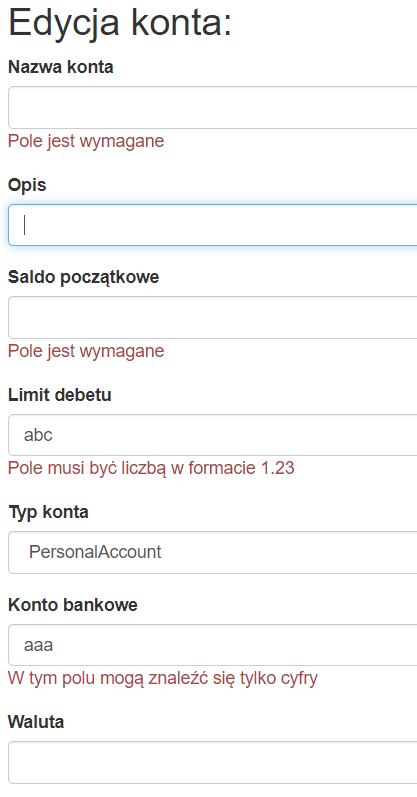
\includegraphics[width=.5\linewidth]{rys05/validation-client-1.PNG}
	\caption{Walidacja danych wejściowych przy tworzeniu konta bankowego}
	\label{fig:client-test-1}
\end{figure}

\section{Testy API}
\label{sec:test-api}

Testowanie API różni się od testowania aplikacji klienckiej. Z racji bycia interfejsem programistycznym i swojej charakterystyki API ma możliwość obsłużyć więcej różnorodnych żądań, niż generuje aplikacja kliencka. 

API też nie powinno ufać klientowi, który z niego korzysta i walidować poprawność danych przychodzących do niego. W razie potrzeby powinno też informować klienta o błędach, poprzez zwrócenie odpowiedniego status błędu HTTP i komunikatu w ciele odpowiedzi.

Poniżej opisano kilka przykładowych przypadków testowych dla API. Na rysunku~\ref{fig:api-test-1} pokazano przykład zwróconego przez API komunikatu o błędzie dla scenariusza testowego VI.

\begin{enumerate}[labelwidth=1em,label=\Roman*]
\item 
    \textbf{Tytuł:} Pobranie wszystkich kont bankowych użytkownika bez podania tokenu dostępu \newline
    \textbf{Kroki reprodukcji:}  \begin{enumerate}[label=\arabic*.]
        \item Adres żądania GET ustawić na na adres \texttt{api/odata/money-accounts}
    \end{enumerate}
    \textbf{Oczekiwany rezultat:}  Serwer zwraca status: \texttt{401 Unauthorized}. \newline
\item 
    \textbf{Tytuł:} Pobranie wszystkich kont bankowych użytkownika \newline
    \textbf{Warunek wstępny:} Klient wysyła w żądaniu token dostępu. Klient komunikuje się protokołem HTTPS. \newline
    \textbf{Kroki reprodukcji:}  \begin{enumerate}[label=\arabic*.]
        \item Do budowanego żądania dodać poprawny \texttt{Beraer} token 
        \item Wysłać żądanie HTTPS GET na adres \texttt{api/odata/money-accounts}
    \end{enumerate}
    \textbf{Oczekiwany rezultat:}  Zwrócenie pól: id, userId, name, description, currency, bankAccountNumber, balance, debitLimit wszystkich kont należących do użytkownika. Kod odpowiedzi serwera: 200. \newline
\item 
    \textbf{Tytuł:} Pobranie wszystkich kont bankowych użytkownika przez protokół HTTP  \newline
    \textbf{Warunek wstępny:} Klient wysyła w żądaniu token dostępu \newline
    \textbf{Kroki reprodukcji:}  \begin{enumerate}[label=\arabic*.]
        \item Do budowanego żądania dodać poprawny \texttt{Beraer} token 
        \item Wysłać żądanie HTTP GET na adres \texttt{api/odata/money-accounts}
    \end{enumerate}
    \textbf{Oczekiwany rezultat:}  Serwer nie odpowiada na żądanie HTTP \newline
\item 
    \textbf{Tytuł:} Pobranie nazw i sald wszystkich kont bankowych użytkownika \newline
    \textbf{Warunek wstępny:} Klient wysyła w żądaniu token dostępu \newline
    \textbf{Kroki reprodukcji:}  \begin{enumerate}[label=\arabic*.]
        \item Do budowanego żądania dodać poprawny \texttt{Beraer} token 
        \item Adres żądania GET ustawić na na adres \texttt{api/odata/money-accounts}
        \item Do adresu żądania dopisać ścieżkę wyszukiwania
    \end{enumerate}
    \textbf{Oczekiwany rezultat:}  Zwrócenie pól: name, balance kont należących do klienta. Kod odpowiedzi serwera: 200. \newline
    \textbf{Dane testowe:} Ścieżka wyszukiwania: \texttt{?\$select=name,balance}.
\item 
    \textbf{Tytuł:} Stworzenie nowego konta bankowego użytkownika \newline
    \textbf{Warunek wstępny:} Klient wysyła w żądaniu token dostępu \newline
    \textbf{Kroki reprodukcji:}  \begin{enumerate}[label=\arabic*.]
        \item Do budowanego żądania dodać poprawny \texttt{Beraer} token 
        \item Adres żądania POST ustawić na na adres \texttt{api/money-accounts}
        \item Do ciała żądania dodać konieczne pola w formacie JSON
    \end{enumerate}
    \textbf{Oczekiwany rezultat:}  Status odpowiedzi serwera: \texttt{201 Created}, wraz z nagłówkiem \texttt{Location}: \texttt{.../api/money-accounts/6e8e0853-0221-43bf-e365-08d7ab0cb343} i zwróconą reprezentacją wysyłanego obiektu. \newline
    \textbf{Dane testowe:} 'userId': '95ab40f9-4ac3-43cb-aeb7-883457f590c8', 'name': 'Konto Millenium Pawel', 'description': 'Moje konto osobiste', 'currency': 'PLN', 'bankAccountNumber': '28124042145653290872967340', 'balance': 4.23, 'debitLimit': 0.00.
\item 
    \textbf{Tytuł:} Stworzenie nowego konta bez podania nazwy \newline
    \textbf{Warunek wstępny:} Klient wysyła w żądaniu token dostępu \newline
    \textbf{Kroki reprodukcji:}  \begin{enumerate}[label=\arabic*.]
        \item Do budowanego żądania dodać poprawny \texttt{Beraer} token 
        \item Adres żądania POST ustawić na na adres \texttt{api/money-accounts}
        \item Do ciała żądania dodać konieczne pola w formacie JSON z wyjątkiem pola \texttt{name}
    \end{enumerate}
    \textbf{Oczekiwany rezultat:}  Status odpowiedzi serwera: \texttt{400 Bad Request}W w ciele odpowiedzi JSON informacą na temat błędu. \newline
    \textbf{Dane testowe:} 'userId': '95ab40f9-4ac3-43cb-aeb7-883457f590c8', 'description': 'Moje konto osobiste', 'currency': 'PLN', 'bankAccountNumber': '28124042145653290872967340', 'balance': 4.23, 'debitLimit': 0.00.
\end{enumerate}

\begin{figure}[t]
	\centering
	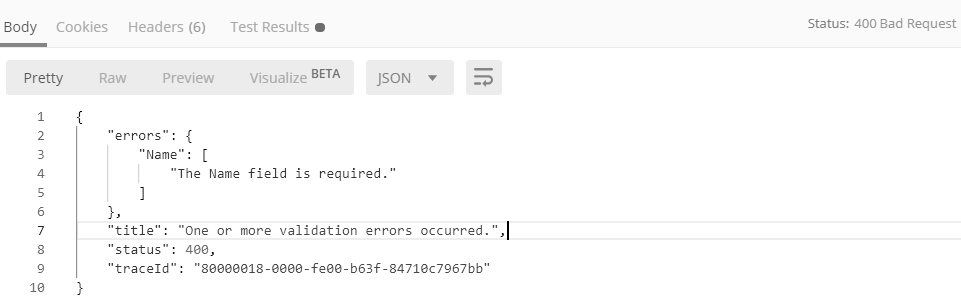
\includegraphics[width=.8\linewidth]{rys05/api-error.png}
	\caption{Przykład odpowiedzi API na błędne żądanie w narzędziu POSTMAN}
	\label{fig:api-test-1}
\end{figure}